% -----------------------------------------------------------------------------
% Master thesis in the study program computational mechanics
%
% B.Sc. Rezha Adrian Tanuharja - 03751261
% M.Sc. Felix Schneider (supervisor)
%
% chapters/discussion/substructuring/point_B.tex
% Last edited 03 November 2023
% -----------------------------------------------------------------------------

\subsection{Vertical Acceleration at Node B}
\label{ssec: cms point B}

Figures \ref{FRF_MC_B_A_linear} and \ref{FRF_MC_B_A_log} show the vertical acceleration magnitudes at node B when a unit vertical force is present at node A.
\begin{figure}[H]
    \centering
    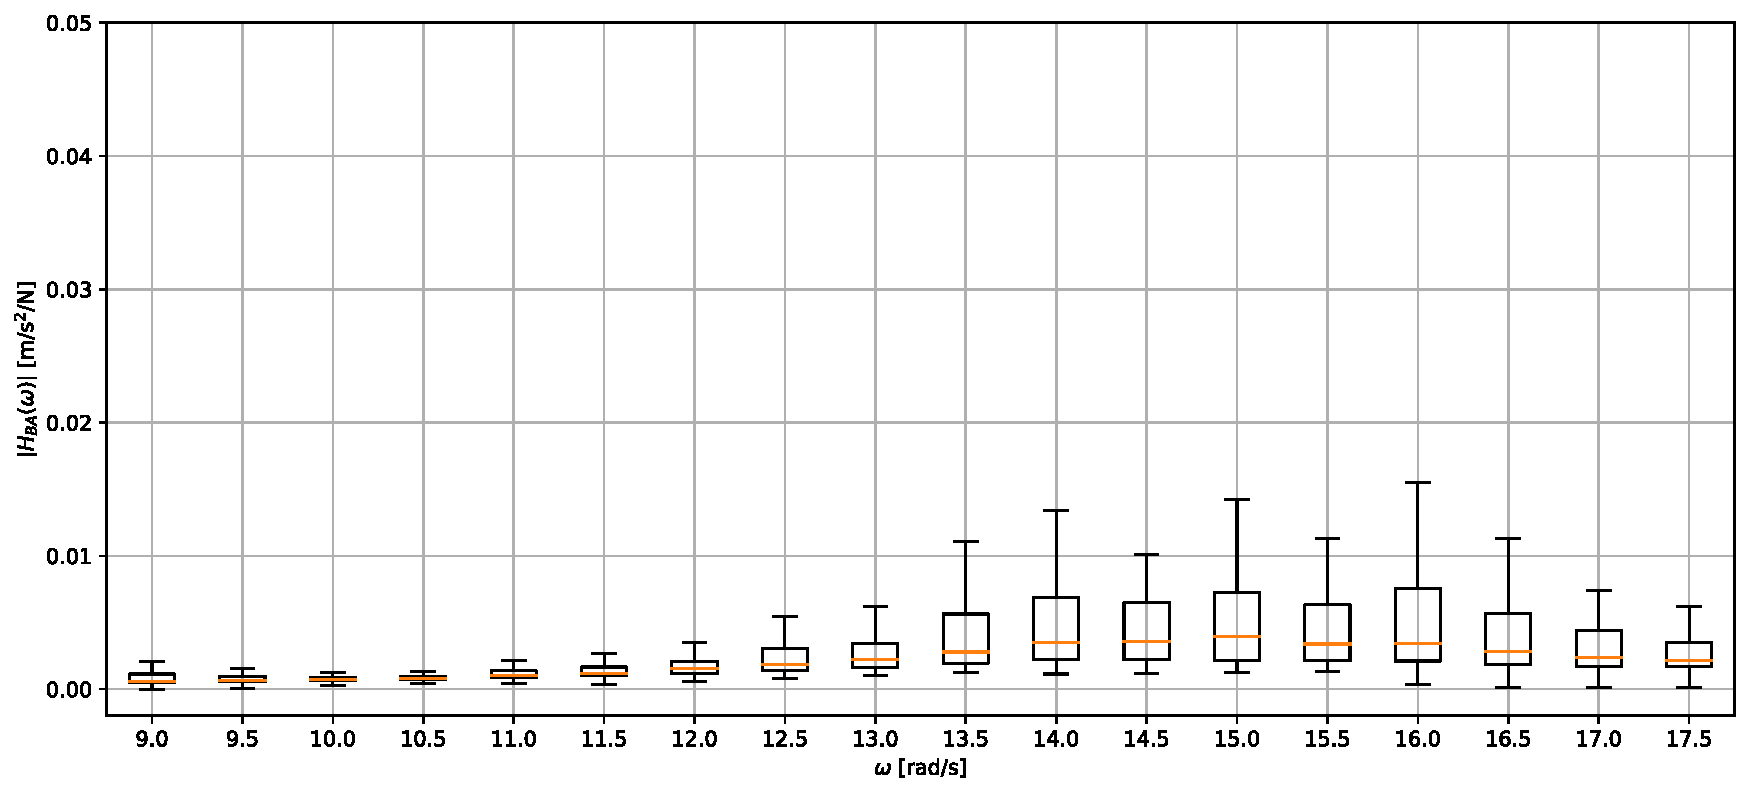
\includegraphics[width=1.0\textwidth]{
        plots/substructuring/plot_8_linear.pdf
    }
    \caption{%
        $\left|H_{BA}\right|$ from Direct MCS of The Complete Plate Model
    }
    \label{FRF_MC_B_A_linear}
\end{figure}
\begin{figure}[H]
    \centering
    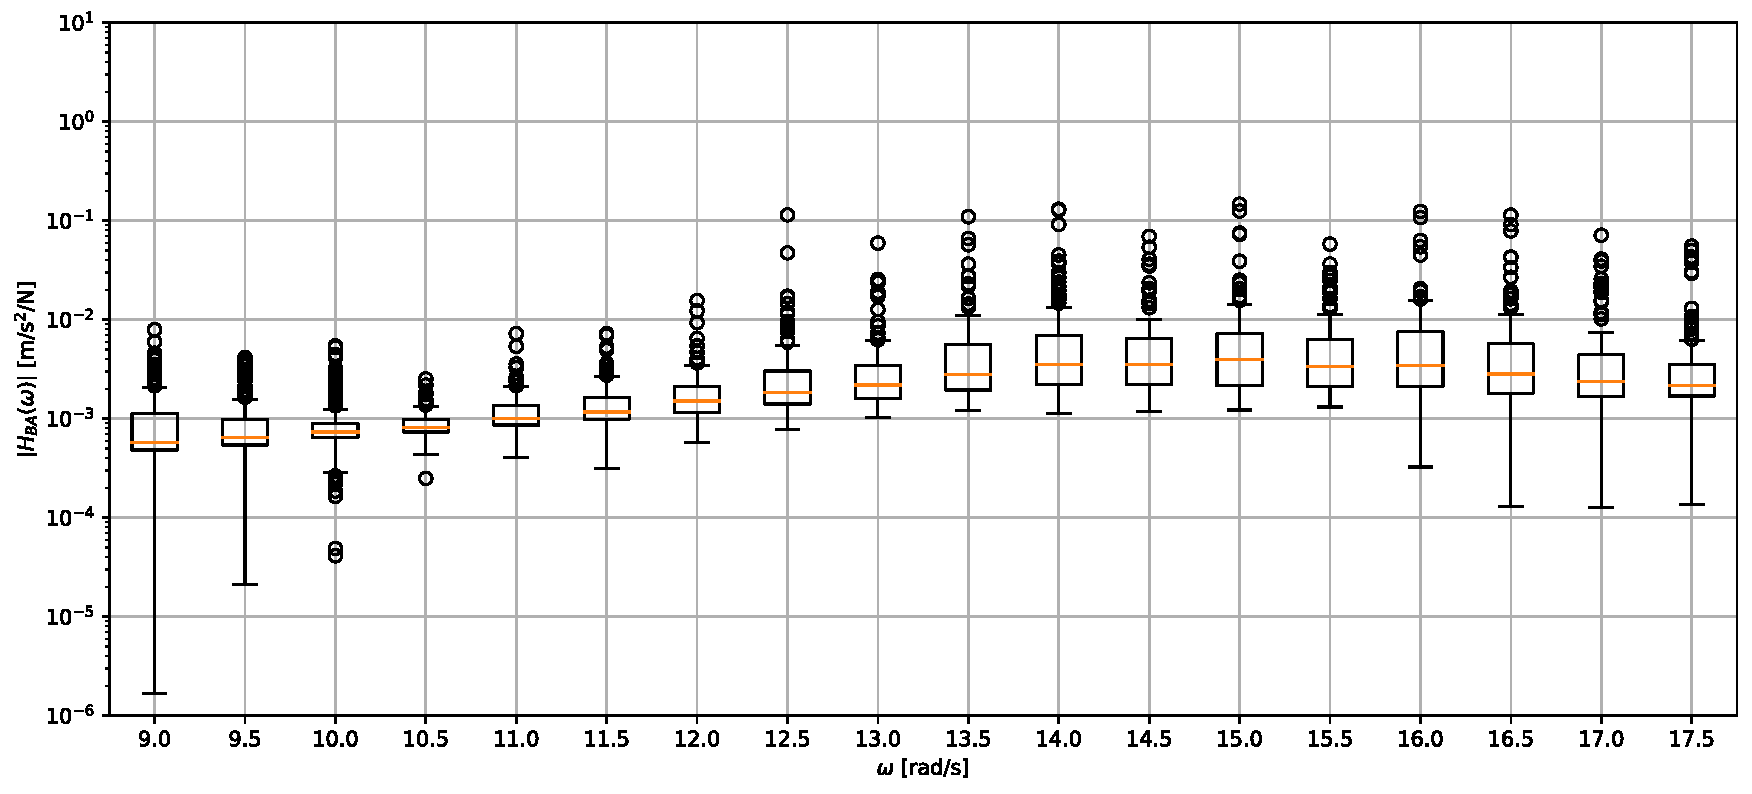
\includegraphics[width=1.0\textwidth]{
        plots/substructuring/plot_8_log.pdf
    }
    \caption{%
        $\left|H_{BA}\right|$ from Direct MCS of The Complete Plate Model with Outliers
    }
    \label{FRF_MC_B_A_log}
\end{figure}
Figure \ref{e_emp CUCB_B_A} shows the median relative empirical errors for the FRFs in each frequency in the above range using three different numbers of internal modes.
The figure exhibits a similar trend with figure \ref{e_emp CUCB_A_A}: as the number of internal modes increases, the relative empirical errors decrease.
\begin{figure}[H]
    \centering
    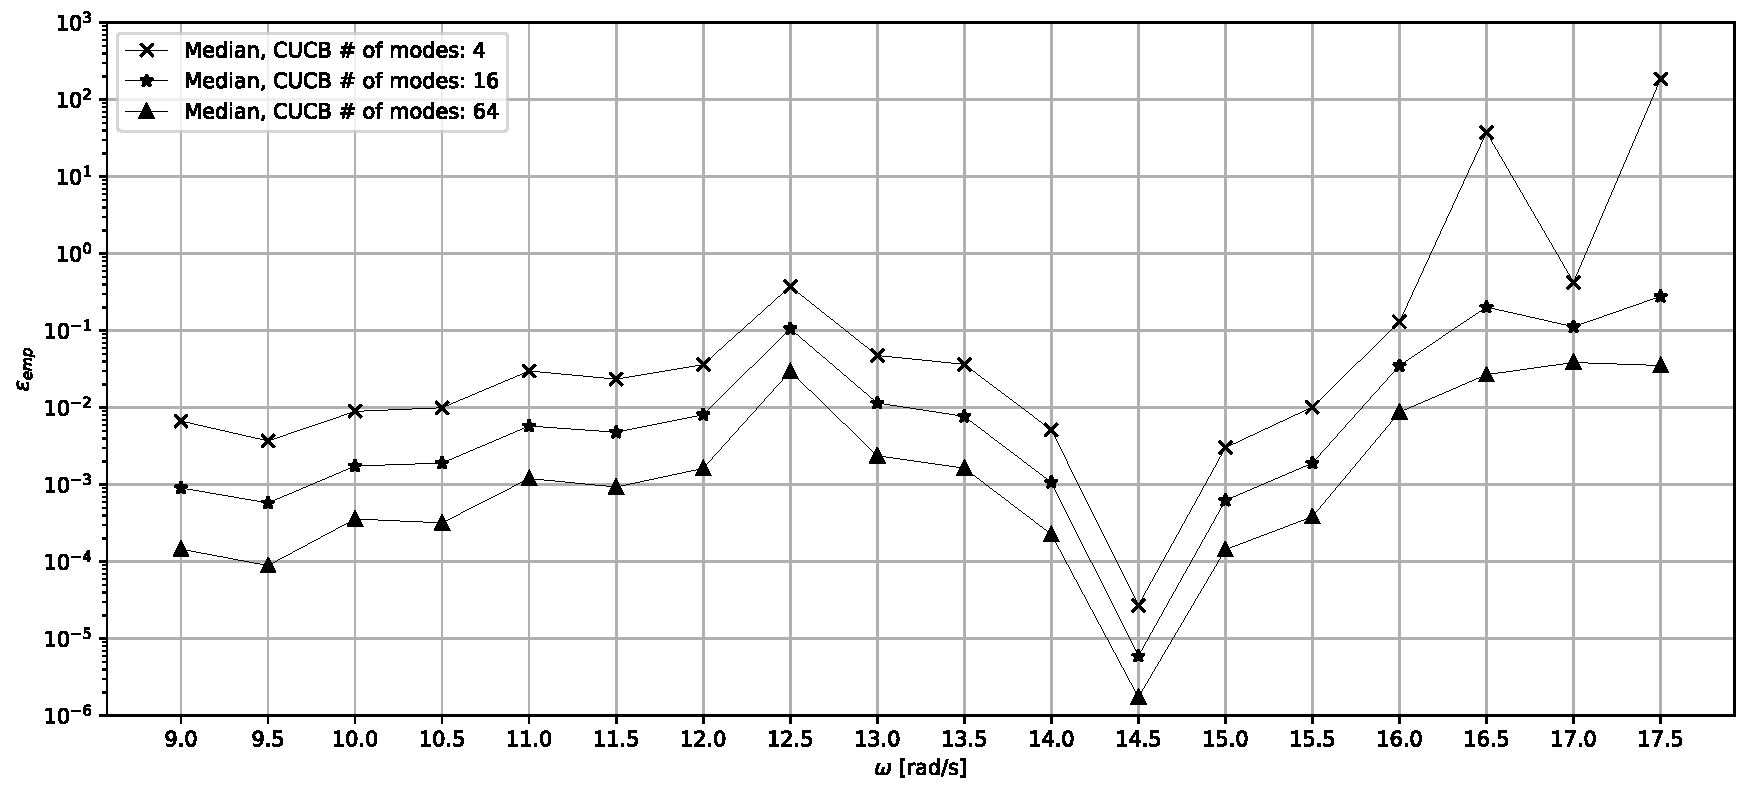
\includegraphics[width=1.0\textwidth]{
        plots/substructuring/plot_9.pdf
    }
    \caption{%
        Relative Empirical Errors of $H_{BA}$ for The CUCB Method
    }
    \label{e_emp CUCB_B_A}
\end{figure}

Figure \ref{e_emp HUCB_B_A} shows the medians and $95\%$ confidence intervals of the relative empirical errors of the FRFs' magnitudes for the crude and hybrid UCB methods.
\begin{figure}[H]
    \centering
    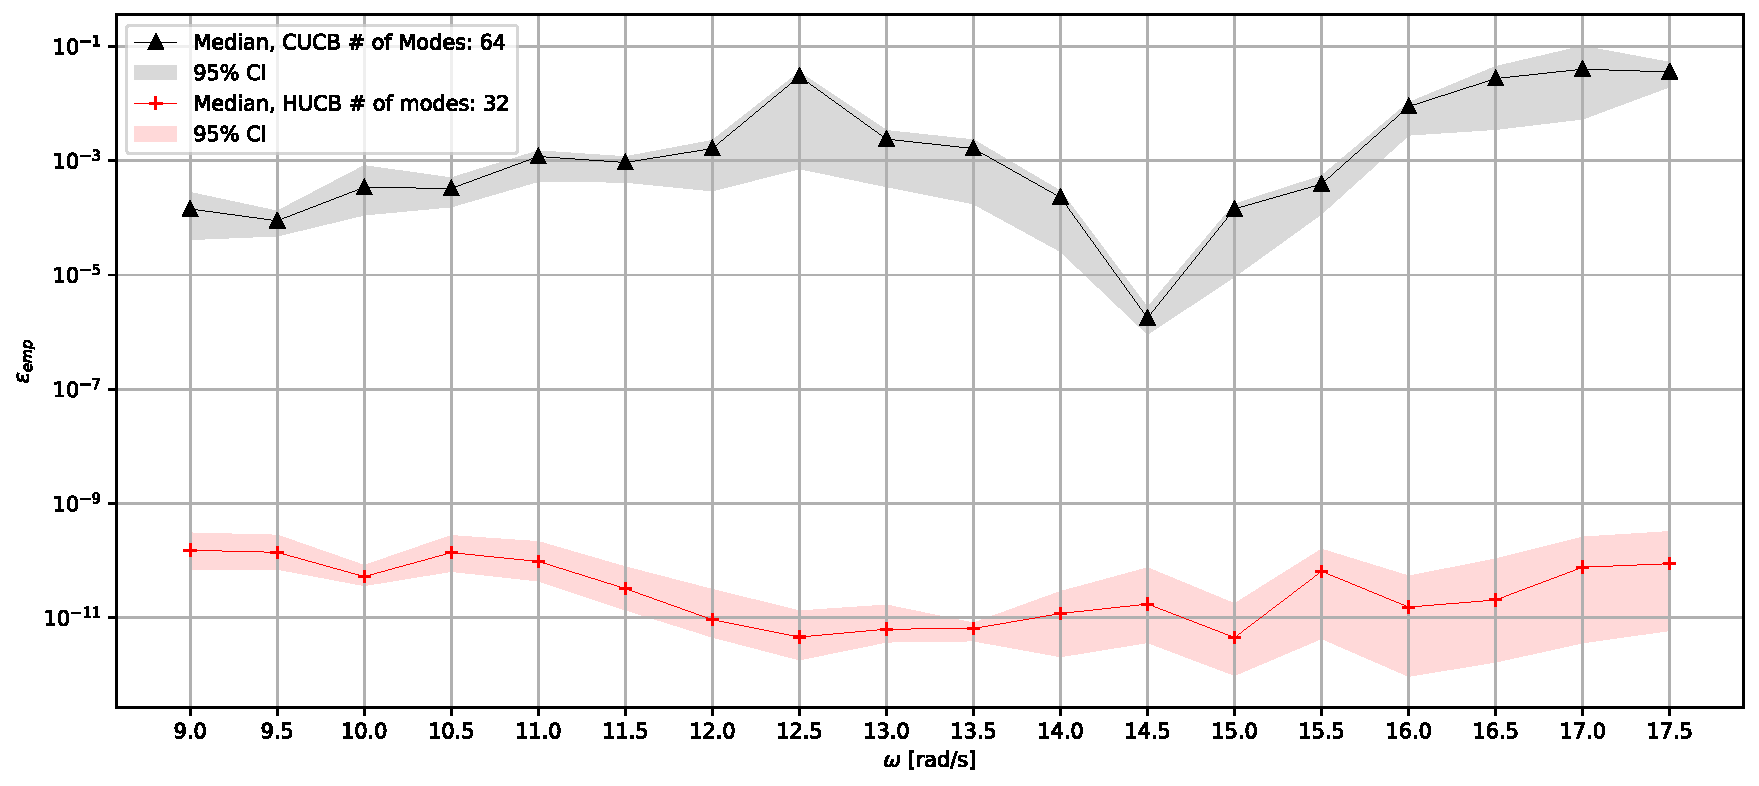
\includegraphics[width=1.0\textwidth]{
        plots/substructuring/plot_10.pdf
    }
    \caption{%
        Relative Empirical Errors of $H_{BA}$ for The CUCB and HUCB Methods
    }
    \label{e_emp HUCB_B_A}
\end{figure}
Comparing figure \ref{e_emp HUCB_A_A} with figure \ref{e_emp HUCB_B_A}, the benefit of the HUCB method over the CUCB method is more pronounced when the force and the response are at two different points or two different components.

Figure \ref{e_mean CUCB_B_A} shows the median relative mean errors of the FRFs' magnitudes for the CUCB method using three different numbers of internal modes.
\begin{figure}[H]
    \centering
    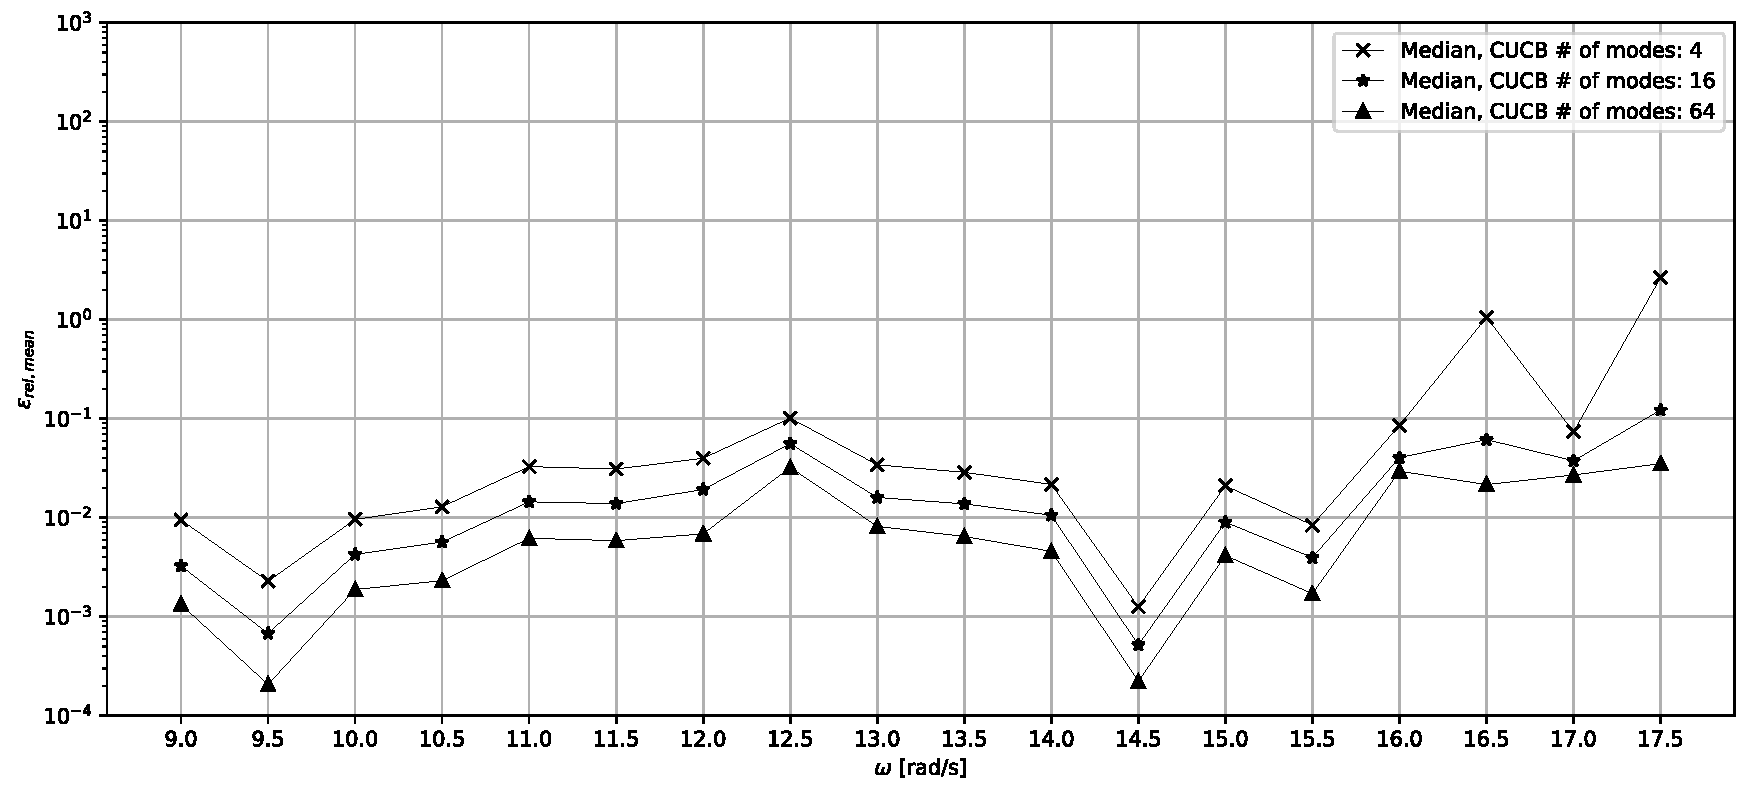
\includegraphics[width=1.0\textwidth]{
        plots/substructuring/plot_11.pdf
    }
    \caption{%
        Relative Mean Errors of $\left|H_{BA}\right|$ for The CUCB Method
    }
    \label{e_mean CUCB_B_A}
\end{figure}
Figure \ref{e_var CUCB_B_A} shows the median relative variance errors of the FRFs' magnitudes for the CUCB method using three different numbers of internal modes.
\begin{figure}[H]
    \centering
    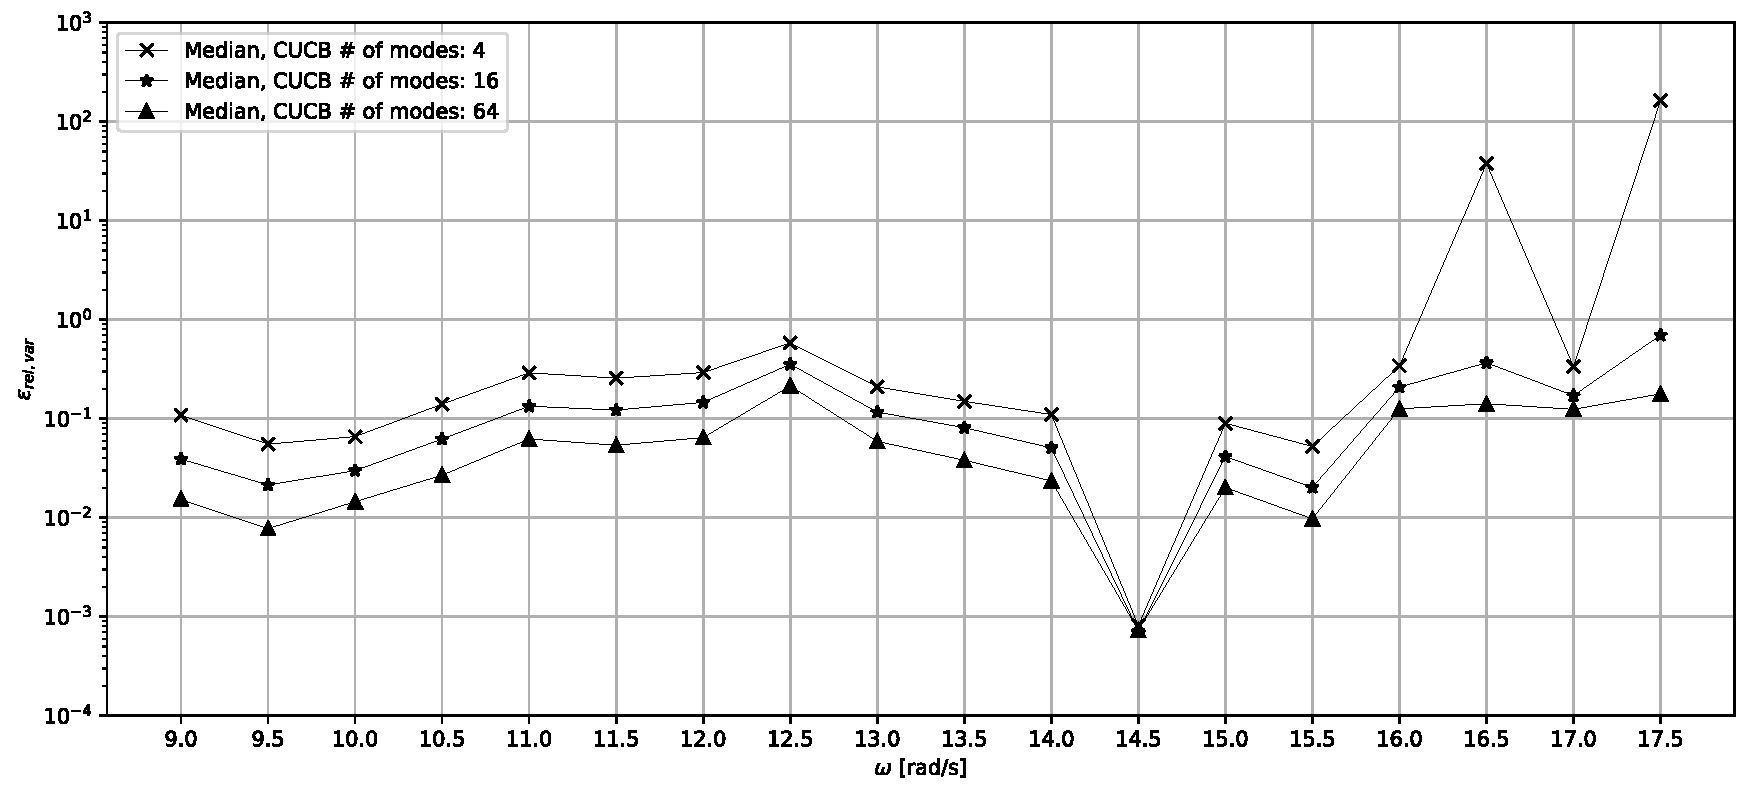
\includegraphics[width=1.0\textwidth]{
        plots/substructuring/plot_12.pdf
    }
    \caption{%
        Relative Variance Errors of $H_{BA}$ for The CUCB Method
    }
    \label{e_var CUCB_B_A}
\end{figure}
The two figures above exhibit similar trends with figure \ref{e_emp CUCB_B_A}: the relative mean errors decrease as the number of internal modes increases.
Overall, the relative mean errors are lower than the relative variance errors.

Figure \ref{e_mean HUCB_B_A} shows the medians and $95\%$ confidence intervals of the relative mean errors for the crude and hybrid UCB methods.
\begin{figure}[H]
    \centering
    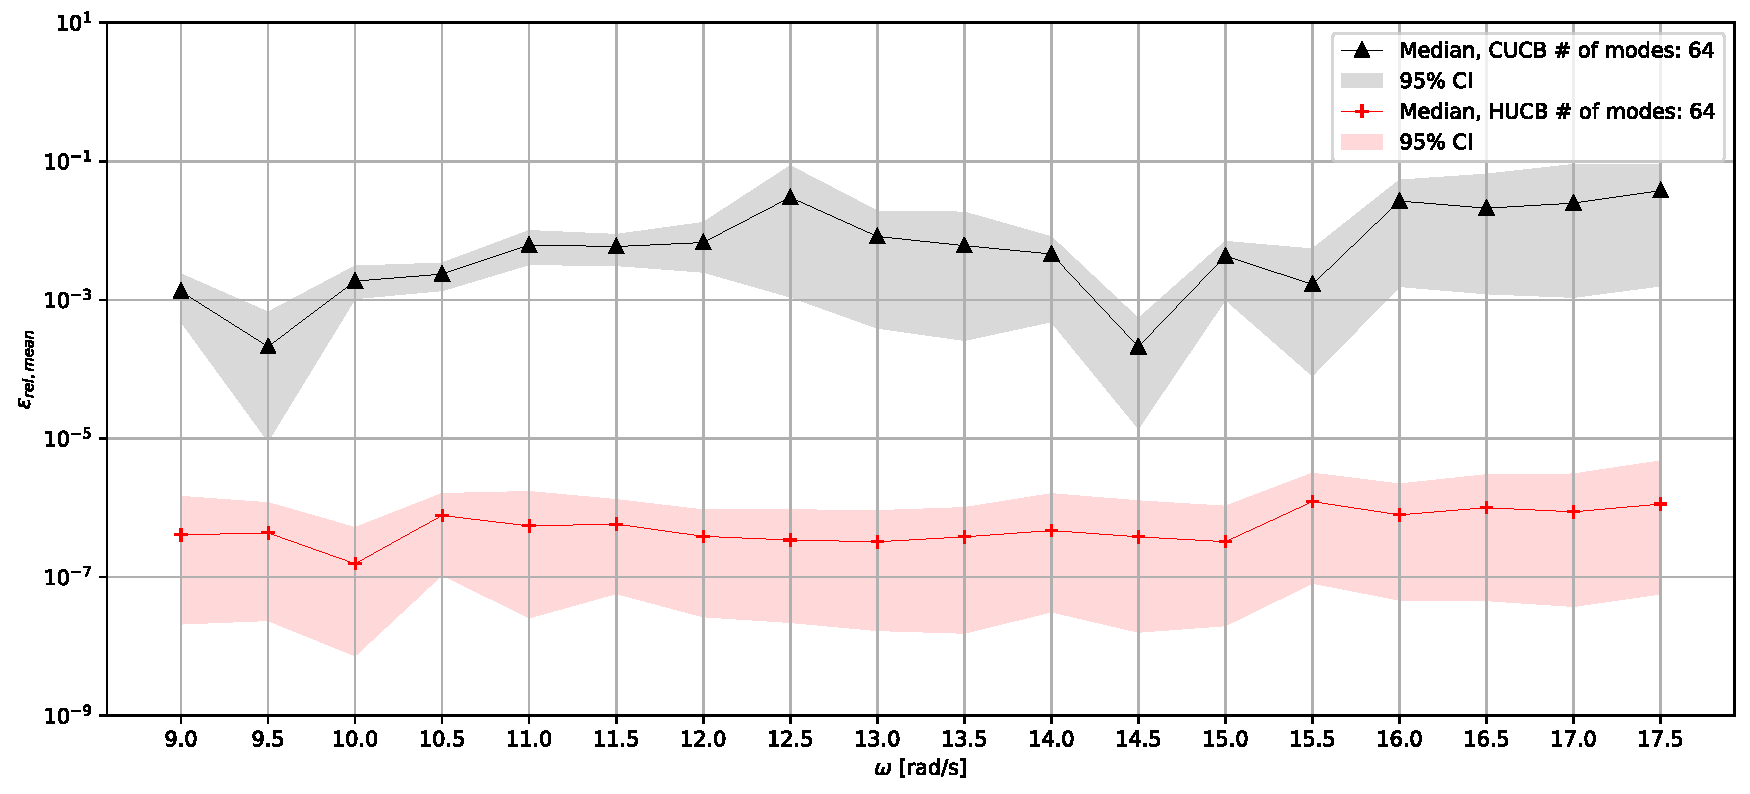
\includegraphics[width=1.0\textwidth]{
        plots/substructuring/plot_13.pdf
    }
    \caption{%
        Relative Mean Errors of $\left|H_{BA}\right|$ for The CUCB and HUCB Methods
    }
    \label{e_mean HUCB_B_A}
\end{figure}
Figure \ref{e_var HUCB_B_A} shows the medians and $95\%$ confidence intervals of the relative variance errors for the crude and hybrid UCB methods.
\begin{figure}[H]
    \centering
    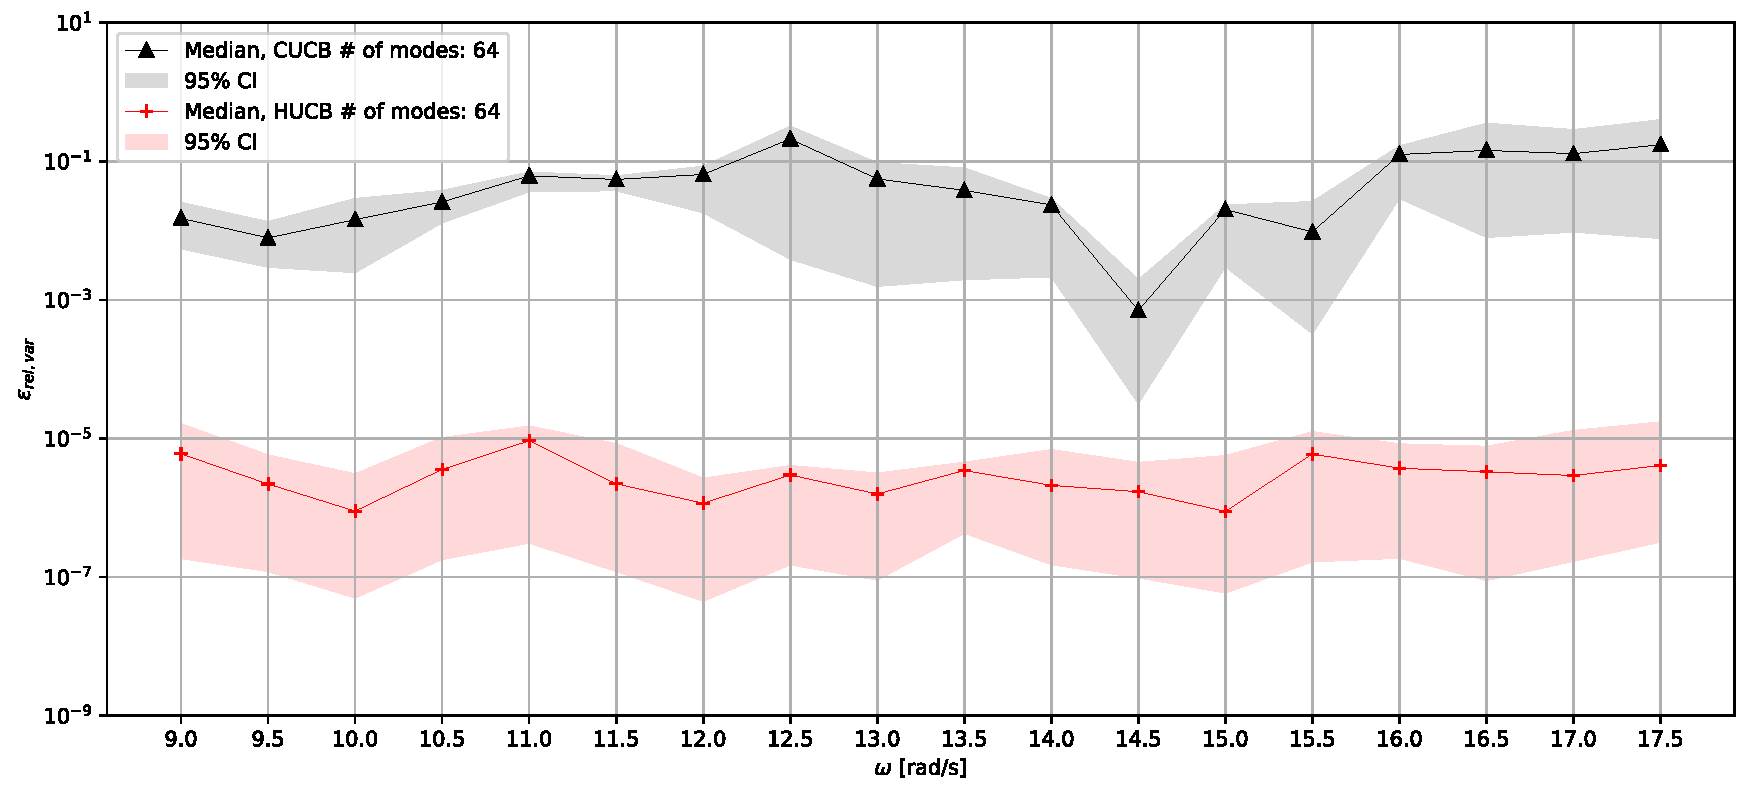
\includegraphics[width=1.0\textwidth]{
        plots/substructuring/plot_14.pdf
    }
    \caption{%
        Relative Variance Errors of $H_{BA}$ for The CUCB and HUCB Methods
    }
    \label{e_var HUCB_B_A}
\end{figure}
The two figures above show that both the relative mean errors and relative variance errors are lower when using the hybrid UCB method by several orders of magnitude.